\documentclass{article}

\usepackage{graphicx}
\usepackage{amsmath}
\usepackage{fullpage}

\begin{document}

\section*{Question 1}

Find the general solution to the below equation using the integrating factor
method.

$$y' + y = 4x + 5x^2$$

Multiply both sides by the integrating factor.

$$\sigma y' + \sigma y = \sigma(4x + 5x^2)$$

Let

$$(\sigma y)' = \sigma y' + \sigma' y = LHS = \sigma y' + \sigma y$$ \hfill (0.5 marks)

So

\begin{align*}
  \sigma ' y &= \sigma y
  \\ \sigma ' &= \sigma
\end{align*}

So $\sigma = e^x$. \hfill (1 mark)

We know

$$(\sigma y)' = RHS = \sigma(4x + 5x^2)$$ \hfill (0.5 marks)

Substituting $\sigma = e^x$

\begin{align*}
  \frac{d e^x y}{dx} &= e^x(4x + 5x^2)
  \\ d e^x y &= e^x(4x + 5x^2) dx
  \\ \int d e^x y &= \int e^x(4x + 5x^2) dx
  \\ e^x y &= \int 4xe^x dx + \int 5x^2e^x dx
  \\ e^x y &= 4 \int xe^x dx + 5 \int x^2e^x dx
  \\ e^x y &= 4 (xe^x - \int e^x dx) + 5(x^2e^x - \int 2xe^x dx)
  \\ e^x y &= 4 (xe^x - e^x + C) + 5(x^2e^x - 2(xe^x - e^x + D))
  \\ e^x y &= 4xe^x - 4e^x + 5x^2e^x - 10xe^x + 10e^x + E
  \\ y &= 4x - 4 + 5x^2 - 10x + 10 + \frac{E}{e^x}
  \\ y &= 5x^2 - 6x + 6 + \frac{E}{e^x} \tag{2 marks}
\end{align*}

So $y = 5x^2 - 6x + 6 + \frac{E}{e^x}$ is the general solution. \hfill (1 mark)

\section*{Question 2}

Use seperation of variables to find the general solution. Then
obtain the particular solution satisfying the given initial condition.
Sketch the graph of the solution, showing the key feaures, and label any
key values.

$$y' = \frac{y}{3x+1}, y(0) = 2$$

\noindent
Separate variables to find the general solution:
\begin{align*}
\frac{dy}{dx} &= \frac{y}{3x+1}
\\ \frac{dy}{y} &= \frac{dx}{3x+1}
\\ \int \frac{dy}{y} &= \int \frac{dx}{3x+1}
\\ \ln \left|y\right| &= \frac{1}{3} \ln \left|3x+1\right| + c
\\ y &= ce^{\frac{1}{3} \ln \left|3x+1\right|}
\\ y &= c \left|3x+1\right|^{\frac{1}{3}} \tag{2 marks}
\end {align*}
Substituting the initial condition, we get,
$$y = 2\left|3x+1\right|^{\frac{1}{3}}$$ \hfill (1 mark)

\noindent
The equation is plotted below. Special points to note include: x-intercept at $\frac{-1}{3}$, the given initial condition $y(0) = 2$, symmetric about $x=\frac{-1}{3}$,and $y->\infty$ as $x->\infty$ and $x->-\infty$. \hfill (2 marks)
\begin{center}
  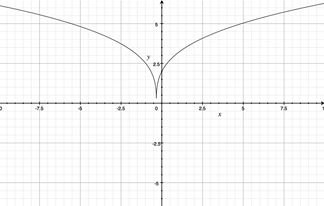
\includegraphics[scale=0.5]{Plot}
\end{center}

\end{document}
